\chapter{\cachename\ Design and Mechanisms} \label{chap:hashcache}
In this chapter, we describe the details of \cachename\ design and the workings of the different \cachename\ mechanisms.
\section{\cachename\ Design} \label{design}
In this section, we describe our organization of the DRAM cache for IHS architectures. The DRAM cache is the first level shared cache between the memory hierarchies of CPUs and GPUs. The CPU cores share a SRAM L2 cache of 1MB among themselves while GPU cores share a SRAM L2 cache of 512KB among them homogeneously. \cachename\ adapts an aggressive direct mapped cache design with tags stored in DRAM as TAD units i.e., Alloy Cache as described in Section \ref{alloy-background}, with a cache line size of 128 byte. We first state and rationalize these design decisions.

\subsection{Metadata Overhead}
The metadata requirement for DRAM caches, even for caches of size 64MB, is large and in the order of few MBs as discussed in Section \ref{dramcache-background}. For example, the metadata of 4MB is required to be stored for a 64MB cache size assuming 128 byte block size and 8 byte metadata per cache block. These metadata sizes are  already in the range of the capacities of last level SRAM caches on modern multicore processors. With DRAM cache sizes projected to be in the order of few Gigabytes in the next few years, this metadata requirement problem poses a significant challenge. The large storage requirement along with the associated cost if it has to be stored in SRAM, has driven DRAM cache designs to either use larger block sizes (of size 2KB or 4KB \cite{footprint,unison-cache}) to reduce metadata overhead or co-locate metadata alongside data in the DRAM cache \cite{loh-hill,alloy,atcache}. 
In the former case, misses waste precious off-chip bandwidth in the absence of spatial locality while the latter design faces slow tag matches.
\par To understand the spatial locality characteristics of large blocks in a IHS configuration, we experimented with 512 byte block organization for the DRAM cache. The 512 byte block size has been shown to provide a good trade-off between increased hit rates and reduced metadata. Earlier studies on DRAM cache designs for multi-core CPUs \cite{bimodal} also favour 512 byte block size, and hence we limit the block size exploration study upto 512B bytes. For DRAM caches that use large block sizes without footprint prediction the larger block sizes are unlikely to give any additional benefits, other than reduction in tag-match delay (due to SRAM tag caches).  However since we are considering direct-mapped Alloy Cache, the tag lookup overhead is unlikely to give any additional benefit. While we increase the cache line size of the DRAMCache, the higher caches (CPU and GPU L2) still operate at 128 byte cache line size i.e. requests to and responses from the DRAMCache are for 128 byte cache lines. Thus one 512 byte cache block in the DRAMCache has four 128 byte sub-blocks that can be requested by higher level caches. When a requested cache line is not found in the DRAMCache, a request for the corresponding 512 byte aligned cache block is sent to DRAM memory. Bringing in a larger block (512 bye) can improve the cache hit ratio (due to spatial locality), the miss penalty (of the DRAMCache) also increases due to the increased fetch and data transfer.
%However, the tag for the sub-blocks is stored for every 128 byte block separately. This simple organization achieves the benefits of a single access for tag-and-data \cite{alloy} for cache lookups, albeit at the cost of some wasted storage for the replicated tags. 
\par We evaluate how much of the data brought by the DRAMCache is actually used by the higher level caches in this setup. We find that on an average for 65\% of the 512B blocks that are brought into the cache, at most 2 sub blocks of 128 byte are requested/used. This implies wasted capacity in the DRAMCache and wasted off-chip bandwidth.
Figure \ref{fig:design-bigblock} on the primary y-axis (left), shows the performance of CPU and GPU using 512 byte block DRAM cache normalized to the performance of 128 byte block DRAM cache. We observe that the 512 byte block consistently under performs the 128 byte block DRAM cache by 12.2\% and 10.6\% for the CPU and GPU respectively in Figure \ref{fig:design-bigblock}. The secondary y-axis (right), shows the increase in the average memory access latency in percentage for a 512 byte block DRAM cache as compared to a 128 byte DRAM cache. We observe that despite a 11\% and 8\% improvement in hit rate in the DRAM cache for CPU and GPU respectively the average memory access latency increases by an average of 75\% for the 512 byte block cache. The increased hit rate comes at the cost of wasted bandwidth and increased off-chip DRAM latency as some of the sub blocks fetched are not used. This study indicates a smaller block size for DRAM cache (\textasciitilde128 bytes) would perform well for IHS workloads.
\par As discussed in Section \ref{dramcache-background}, Tags-in-DRAM designs have further focused on improving access latencies by removing tag-serialization overhead using overlapped tag lookups \cite{loh-hill} or storing TAD units \cite{alloy}. These designs come close to tags-in-SRAM like access latency without concerns of spatial locality characteristics of large block sizes. Further, using a non-standard burst length tags can even be retrieved along with data for no additional latency overhead from the stacked DRAM cache.
\par Hence, \cachename\ organizes data at 128 byte block size and stores data in DRAM cache as a cohesive TAD unit.

\begin{figure}[htbp]
   \centering
   \includegraphics[scale=1.05]{graphs/design-bigblock}
   \caption{Performance of 512B vs 128B block size}	
   \label{fig:design-bigblock}
\end{figure}

\subsection{Associativity} 
Providing set associativity is known to improve cache hit rates by reducing conflict misses. In DRAM caches where tag is stored in DRAM,  associativity comes at a cost. Hit latencies increase due to the tag requiring to be burst out of the stacked DRAM. Hence there is an implicit trade-off between providing better hit-rates and reduced access latency. As shown in Section \ref{motivation} (Figure \ref{fig:motivation-gpu-cache}), a higher associativity design is suitable for a GPGPU processor which can trade increased access latency for higher hit rates to make better use of the larger bandwidth of the DRAM cache. On the other hand, the CPU would suffer when using such a design due to the increased hit-latency, and  would instead prefer a latency-optimized direct-mapped cache \cite{alloy}.
\par The large performance decline for CPUs due to co-running requires \cachename\ to be organized as a direct mapped cache to achieve better hit time for improved CPU performance. Further, such a direct mapped organization simplifies the design and eschews the need for tag-caches \cite{atcache} and way locators \cite{bimodal} to improve hit times. \cachename's organization is also inline with the commercially adopted stacked MCDRAM on the Knights Landing generation of the Intel XeonPhi processor \cite{xeonphi} where the DRAM cache is organized as a direct mapped cache.

\subsection{Miss Penalty}
Past research works in stacked DRAMs have assumed an access latency which ranges from 0.5x to 1.0x of off-chip DRAM, while recent data sheets advocate a value closer to 1.0x, especially for large capacity stacked DRAM of close to 1GB. In our work, with a smaller stacked DRAM size of 64MB and 128MB, we assume an access latency of 0.7x compared to the off-chip DRAM latency. Even with this latency, a miss in the DRAM cache would experience a delay of 1.7x as the DRAM (memory) access takes place after the miss is detected (serially). To overcome this, researchers have proposed cache line hit predictors \cite{loh-hill,alloy} which are critical to extract performance from DRAM caches. These predictors start an early access to memory if they predict that the block will miss in the DRAM cache. Starting an early access to off-chip main memory can remove the DRAM cache lookup serialization and effectively overlap some of memory access latency with the DRAM cache tag lookup.
\par Intuitively, we apply the MAP-I prediction (Instruction Based Memory Access Predictor) \cite{alloy} to CPU requests to start early memory access when an access is predicted to be a miss. The MAP-I mechanism works by using the address of the instruction (Program Counter) making the access to the DRAM cache to make a prediction about a hit or miss. Such a correlating predictor has been shown to have reasonable accuracy of about 95\% for multi-core CPUs \cite{alloy}. For GPUs, the MAP-I predictor is not used and the requests always proceed serially through the cache after verifying via tag match. This helps to (a) reduce the wastage of off-chip bandwidth for mis-predictions for GPU (b) avoid large structures that will be required for making reliable predictions for GPUs which might require correlating warp, thread, and CU IDs.

\subsection{Row Buffer Hits (RBH) vs Bank Level Parallelism (BLP)} 

Stacked DRAMs, similar to commodity off-chip DRAMs, are organized as vaults (channels), layers (ranks) and banks within each layer as shown in Figure \ref{fig:stackdram}. This organization is similar to that of off-chip DRAMs as explained in Chapter \ref{chap:background}. Each vault has several TSVs which constitute lanes in a channel. Each layer shares a command, address and data bus and each bank is  operated and accessed independently. As discussed in Section \ref{dram-background}, DRAMs exploit this parallelism, called Bank Level Parallelism (BLP), to improve effective memory bandwidth. Given this abundant BLP in stacked DRAMs, we ask the question should DRAM caches addressing scheme favour exploiting this parallelism over improved RBH? In other words, we ask the question should the addressing scheme of a DRAM cache be organized as RoCoRaBaCh (Row,Column,Rank,Bank,Channel) --- referred to as the BLP-scheme --- which distributes a cache block in banks of different ranks as opposed to RoRaBaCoCh --- referred to as the RBH-scheme --- which stores cache blocks consecutively in the row of a bank. We experimented with both the addressing schemes for an IHS processor with a DRAM cache. Figure \ref{fig:design-rbhblp} shows the performance of a DRAM cache that uses a BLP addressing scheme normalized to the performance of a RBH addressed DRAM cache. We observe that both the CPU and GPU applications experience on an average 3\% and 1\% lower H-Mean IPC respectively when using the BLP scheme. Hence we choose the RBH friendly addressing scheme (RoRaBaCoCh scheme) to address \cachename.
\begin{figure}[!htb]
	\centering
	\includegraphics{graphs/design-rbhblp}
	\caption{Performance of BLP-scheme vs RBH-scheme}
	\label{fig:design-rbhblp}
\end{figure}

\par To summarize, our \cachename\ organizes DRAM cache as follows
\begin{itemize}
	\item 128 byte block size with tags stored in DRAM rows (tags-in-DRAM)
	\item Direct Mapped DRAM cache with a longer burst length to retrieve tag along with data
	\item Early Memory access predictor for CPU requests, while GPU proceed serially via tag match
	\item Uses an addressing scheme that attempts to maximize row buffer hits
\end{itemize}


\section{\cachename\ Mechanisms}

As noted in Figure \ref{fig:motivation}, despite the addition of such a carefully designed DRAM cache, the CPU applications when run along with GPU applications in an IHS architecture do not achieve the full benefits of the DRAM cache compared to when they are run alone. The GPU applications on the other hand are relatively unaffected by the co-running of CPU applications. This can be attributed to the GPUs capability to context switch among warps to make it latency tolerant. This suggests that the DRAM cache should be optimized to regain the lost CPU performance without compromising the GPU performance. In this section we propose three schemes for achieving this. For each mechanism we state the objective and then articulate its working.

%-----------------------------------------------------------%

\subsection{Heterogeneity-Aware DRAM cache Scheduling} 
\textbf{Objective:} Reduce the large access latencies for CPU requests at DRAM cache
\subsubsection{Premise}
In an IHS architecture, the CPU requests experience bursts of requests from the co-running GPU application. The imbalance in request arrival rates between CPU cores and GPU cores causes a significant increase of 113\% on an average, in memory access latency for CPU requests as observed earlier in Figure \ref{fig:motivation-cpu-cache}. This increase in memory access latency causes the CPU performance to decrease as compared to when it ran alone without the co-running GPU workload.
\par As detailed in Chapter \ref{dram-background}, DRAM devices have traditionally had limited size queues to hold requests until they can be serviced by the device. However, we observe that in an IHS processor the large burst of requests from the GPU quickly exhausts the limited size buffer (meant for holding the requests till they are serviced) at the DRAM cache controller. This leads to requests being rejected causing the DRAM cache to be blocked. 
The CPU requests, which are interleaved with the GPU requests, are few and far spaced and thus suffer large waiting time due to retries. This is further compounded by the fact that GPU exploits good row buffer locality and is preferentially scheduled by the DRAM cache controller (under FR-FCFCS scheduling \cite{sms}), causing increased queue latencies for CPU requests. Increasing queue lengths beyond a certain measure increases scheduling overheads as DRAM schedulers search the queues for the most suitable request to schedule based on certain heuristics.
\par To reduce this increased access latencies for CPU requests at DRAM cache, we propose a heterogeneity-aware DRAM cache access scheduling mechanism called \prioname\ (CPU Prioritized FR-FCFS with IHS aware Scheduling).

\subsubsection{Mechanism Overview}
\par \cachename\ reduces waiting time of CPU requests by prioritizing them at the DRAM cache controller without starving GPU requests. 
For this, \cachename\ applies a CPU Prioritized FR-FCFS algorithm over each of the Read, Write and Fill queues to schedule a request at each bank. 
The scheduler is cognizant of the request heterogeneity and searches the short queues for either a first CPU row buffer hit request or a first CPU row activation request to schedule before scheduling a GPU request in a FR-FCFS manner. For GPU requests, starvation is avoided firstly, by allowing GPU requests to be scheduled to a prepped (open) row after the CPU has completed access to that row and secondly by allowing GPU to schedule its requests to a bank immediately, when the queue has no more CPU requests to that bank. These scheduling decisions are made subject to the device timing constraints, similar to an FR-FCFS scheduler.
\par Prioritization of CPU requests alone may not help, as the flood of memory requests from  GPU can quickly fill the precious buffer at the DRAM cache controller, resulting in CPU requests not even entering the buffer (queue). \cachename\ overcomes this problem by guaranteeing certain minimum occupancy for CPU requests in the buffer at the DRAM cache Controller. This is accomplished using a selective reject-retry mechanism for GPU requests when the queues reach certain critical level.  Together these two mechanisms attempt to reduce the DRAM cache latency experienced by CPU requests.  We refer to these  mechanisms collectively as \prioname\ (CPU \emph{Pr}ioritized FR-FCFS with \emph{I}HS aware \emph{S}cheduling). 
\par \prioname\ differentiates requests broadly as CPU or GPU requests and not within individual CPU cores or GPU CUs for scheduling. We find that in an IHS architecture the interference between CPU and GPU applications vastly overwhelms the interference between homogeneous application workloads. Hence, \prioname\ only has to make a binary selection for scheduling which greatly simplifies the scheduling algorithm. 

\subsubsection{Hardware Overhead}
\prioname\ is a simple yet effective, single stage modified FR-FCFS algorithm that does not incur any hardware overhead in terms of multiple or large requests queues or batching stages as in \cite{sms}. We also compare the performance of \prioname\ against the mechanism in \cite{sms} subsequently in Chapter \ref{chap:related-work}.

\subsubsection{\prioname\ Algorithm Details}
\par The complete \prioname\ scheduling algorithm is stated in Algorithm \ref{algo-pris}. \prioname\ picks requests to be scheduled from the input queue. The exact selection of input queue (Read, Write or Fill Queue) is done external to this algorithm based on certain heuristics and constraints which is beyond the scope of this scheduler algorithm. Broadly, the algorithm picks one of the 3 types of requests; (a) seamless row buffer hit, (b) hidden bank prep or (c) prepped row, in that strict order of priority. These are explained below.
\par A seamless row buffer hit request refers to a request that can issue a column access to an already activated row in the bank, without any further delay. A hidden bank prep request is a request that can overlap the current operation in other banks (in the same rank) and issue a request to activate or precharge a row in the requested bank. Among the hidden bank prep requests an FCFS policy is followed. A prepped row request refers to a request that needs to wait for the current column access to complete to the currently active row in a bank. Thus choosing a prepped row leads to a bubble in the pipeline of the scheduler where the request has to wait for the row to become available for a column access command.

\par Additionally, the \prioname\ algorithm picks a request in the priority order of
\begin{quote}
CPU seamless row buffer hit $>$ CPU hidden bank prep $>$ CPU prepped row $>$ GPU seamless row buffer hit $>$ GPU hidden bank prep $>$ GPU prepped row buffer hit
\end{quote}
We experimented with several combinations of this priority order and find that prioritizing CPU requests at all levels provides best performance for CPU requests while the reduction in GPU performance due to de-prioritization between the schemes was not significant.
\par Thus, \prioname\ is able to reduce access latencies by reducing waiting delay and queue latencies for CPU requests at DRAM cache.
\begin{algorithm}
	\normalsize
	\KwIn{DRAMCache Queue}
	\KwOut{selected\_req to be scheduled}
	all bool variables are initialize to \textit{false}\\
	%found\_seamless\_gpu\_req = false\\
	%found\_prepped\_req = false\\
	%found\_prepped\_cpu\_req = false \\
	%found\_earliest\_req = false \\
	%found\_earliest\_cpu\_req = false \\
	
	\While{not at end of Queue}{
		read \textit{rank}, \textit{bank} and \textit{row} of current\_req \\
		\If{rank.isAvailable} {
			\uIf{row.isOpen}{
				\uIf{bank.colAllowedAt <= minColAt}{
					\tcc{seamless row buffer hit}
					\uIf{req.isCPU}{
						selected\_req = current\_req \\
						break \\
					}
					\ElseIf{!found\_seamless\_gpu} {
						selected\_req = current\_req \\
						found\_seamless\_gpu = true \\
					}
				} \ElseIf {!found\_hidden\_bank \&\& !found\_prepped\_cpu \&\& !found\_seamless\_gpu} {
				\tcc{req to prepped row}
				\uIf{req.isCPU}{
					selected\_req = current\_req \\
					found\_prepped\_cpu = true \\
					found\_prepped = true \\
				}
				\ElseIf{!found\_seamless\_gpu} {
					selected\_req = current\_req \\
					found\_prepped = true  \\
				}
			}
		} \ElseIf {!found\_earliest\_cpu \&\& !found\_seamless\_gpu} {
		\tcc{earliest bank that can be issued hidden cmd}
		\tcc{executed only once per scheduling decision}
		found\_hidden\_bank, earliest\_bank = find\_earliest\_bank() \\
		\If{earliest\_bank == bank \&\& \\ (found\_hidden\_bank || !found\_prepped)} {
			\uIf{req.isCPU}{
				selected\_req = current\_req \\
				found\_earliest\_cpu = true \\
				found\_earliest = true
			}
			\ElseIf{!found\_seamless\_gpu} {
				selected\_req = current\_req\\
				found\_earliest = true \\
			}
		}
		
	}
}
}
\caption{\prioname\ DRAMCache scheduling policy}
\label{algo-pris}
\end{algorithm}

%-----------------------------------------------------------%

\subsection{Heterogeneity-Aware Temporal Bypass} \label{mechanism-bye}
\textbf{Objective:} Utilize the under-utilized off-chip DRAM Bandwidth
\subsubsection{Premise}
The large sizes of the stacked DRAM cache ensures cache lines have fairly long residency time before being evicted. Hence, DRAM cache has fairly large hit rates which leads to idling of off-chip DRAM bandwidth as shown in Section \ref{motivation}. Moreover the stacked DRAM and off-chip DRAM utilize the same underlying technology and hence incur comparable latency (0.7x for DRAM cache vs 1.0x for DRAM). Thus, directing some requests to off-chip allows improved resource utilization and allows us to exploit the aggregate bandwidth of both DRAM cache and DRAM buses without incurring significant latency overheads.
%i.e. arrays of charge retaining capacitor cells, and hence they incur similar access latencies to read and write to these capacitors. 
\par Further, we take cue from another observation made from requests which are mis-predicted as misses in the DRAM cache. As mentioned in Section \ref{alloy-background}, to hide the latency of miss, our aggressive baseline design already incorporates a hit/miss predictor (similar to MAP-I predictor \cite{alloy}) for CPU requests to initiate an early access to off-chip DRAM when a miss is predicted in the DRAM cache. These requests are then enqueued in the DRAM cache queues for verification of a miss 
\footnote{This is required to ensure that misprediction does not result in using stale data from the DRAM for lines modified (dirty) in DRAM cache}
by a tag match. 

Once the tag is compared (matched) against the requesting address in the DRAM cache either of the following 2 cases ensue: 
\begin{enumerate}[label=(\alph*)]
	\item In the case of a hit, data from the DRAM cache is forwarded to the requester and the DRAM memory access is squashed or its response is ignored. 
	\item In the case of a miss, data from the memory is forwarded and inserted into the cache.
\end{enumerate}
Normally, it is expected that the access to the DRAM cache completes earlier (due to its relatively lower access latency) than the DRAM response. However, when the GPU is running, the parallel request to off-chip DRAM memory often returns earlier and waits in the MSHRs. This is due to the increased queuing delay at the DRAM cache compared to the access latency at the DRAM. \cachename\ exploits this observation to bypass CPU read requests for both misses and clean lines thereby circumventing this waiting delay.
In a IHS architecture, with a co-running GPU application a DRAM cache hit for a CPU request often experiences a latency which is higher than 1.0x of off-chip DRAM memory as shown in Figure \ref{fig:motivation-cpu-cache}. 
This makes the off-chip DRAM an attractive target to direct some of the CPU requests, even those that are likely to be DRAM cache hits. Such a scheme can lead to improved resource utilization of off-chip bandwidth without incurring any increased latencies for CPU requests.
\par To achieve this, we propose a bypass mechanism for CPU requests that are hits to clean lines in the DRAM cache. For correctness reasons, hits to dirty (modified) lines in the DRAM cache should not be bypassed. We call this heterogeneity-aware temporal scheme as \bypassname.


\subsubsection{Mechanism Overview}

\begin{figure}[htb]
	\centering
	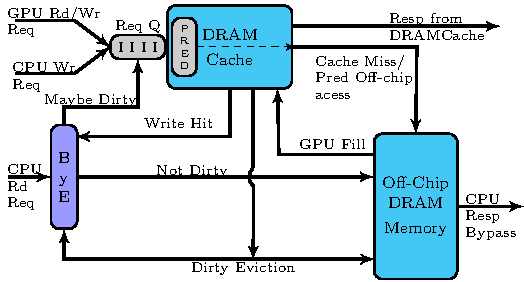
\includegraphics[scale=1.5]{figures/bloom}	
	\caption{Working of \cachename\ with \bypassname}
	\label{fig:bye}
\end{figure}

\par To allow the CPU requests to bypass the DRAM cache, \cachename\ needs to be able to track and lookup dirty lines in the DRAM cache. However, maintaining a list of all dirty lines in the DRAM cache would require prohibitively large storage structures. Thus, \cachename\ uses an approximate tracker called Bypass Enabler (\bypassname). \bypassname\ uses a counting Bloom filter \cite{bloom,counting-bloom} that tracks the dirty lines in the DRAM cache and provides a space efficient way to determine if a given request can be bypassed. The property of a Bloom filter to answer "definitely not in set" allows us to bypass requests correctly i.e., without verifying tags in the set of the DRAM cache. 
On a write request when a cache line becomes dirty in the DRAM cache, the address is hashed into \bypassname\ and the corresponding counters are incremented. When a dirty line is evicted from the DRAM cache, \bypassname\ attempts to remove the entry from the Bloom filter by decrementing the corresponding locations 
\footnote{Counting bloom filters use saturating counters. If counter saturates, decrementing it can lead to false-negatives (dirty lines predicted as clean lines and wrongly bypassed). Hence in our scheme, saturated counters are never decremented.  While this may increase the false positives (clean lines being predicted as dirty), which only reduces the benefits obtained by \textit{ByE}, it does not affect functional correctness. In our implementation we observe that on an average just 2\% of the 2-bit counters in the Bloom-filter saturate out of the 512K counters. Further, saturation of Bloom filter is a cause of concern for large DRAM caches and long running systems. Clearing the filter would require time consuming operation of scrubbing dirty blocks from cache. However, it is possible to design a per rank or a per bank bloom filter. When the bloom filter for a rank or bank saturates (or Bloom filter produces large number of false positive) the corresponding cache lines in the rank or bank can be scrubbed. The rest of the DRAM can continue regular operation. Only the requests corresponding to the rank or bank being scrubbed will face higher latency.}.
\par \bypassname\ bypasses CPU requests only when the GPU cores are executing the kernel. For this, all CPU read requests lookup into \bypassname\ as shown in Figure \ref{fig:bye}. If the Bloom filter search returns a  negative result, then the address is guaranteed to be not dirty in the DRAM cache. Thus, the request can safely be bypassed to utilize the off-chip DRAM bandwidth. 
\par All write requests and GPU read requests proceed serially after looking into the cache. \bypassname\ does not bypass any write requests as it would otherwise require a back-invalidation of the cache line, if present in the DRAM cache, which would need a full DRAM cache access.

\subsubsection{Insertion Policy}
\par Further, when the bypassed CPU requests return from the off-chip DRAM access, these requests are directly forwarded to the requester and are not inserted into the cache. 
Firstly, this allows \bypassname\ to ensure that future write requests for the line do not hit in the DRAM cache as increase in dirty lines would lead to reduced bypass efficiency. 
% (we wanted this sentence cuz we dont want the reader to start thinking of reduced hit rates) Firstly, this allows \bypassname mechanism to continue bypassing future read requests for the line by ensuring that the write requests for  line do not hit in the cache causing reduced bypass efficiency
Secondly, this allows \bypassname\ to reduce some of the bloat caused by a Miss Fill \cite{bear} into the DRAM cache.
Thus, the no-insert policy and the \bypassname\ act as complementary self balancing mechanisms - trading off CPU hit rates in DRAM cache for better access latency at the off-chip DRAM.
\subsubsection{\bypassname\ Hardware Overhead}
\par We find that a small 2-bit counting Bloom filter implemented with two $H_3$ hash functions \cite{h3} and 512K entries per controller is sufficient 
to produce reasonable bypass efficiency with a tolerable misprediction rate. The total overhead for \bypassname\ is 256KB for a 64MB DRAM cache which is less than 0.4\% of the cache size.
\par Thus, \bypassname\ is designed to improve performance by achieving a better bandwidth balance between the DRAM cache and the off-chip main memory.

%-----------------------------------------------------------%

\subsection{Heterogeneity-Aware Spatial Occupancy Control} \label{mechanism-chaining}
\textbf{Objective:} Allow GPU to better use DRAM cache Bandwidth
\subsubsection{Premise}
The schemes proposed in the previous two subsections, \prioname\ and \bypassname, attempt to improve the latency of CPU requests. The mechanism described in this section details \cachename's approach to improve the utilization of the DRAM cache for GPU requests, in order to exploit the higher bandwidth provided by it. 
\par First, we make the following observations and inferences: 

\begin{enumerate}[label=(\roman*)]
	\item The working sets of CPU applications tend to be limited to few tens of MBs due to the limited amount of MLP that can be exploited by the CPUs. Thus, providing larger than certain share of cache leads to no further improvements in hit rates and IPC for CPU. Nevertheless, the CPU can still gain from some share of the DRAM cache due to reduced latency of access.
	\item Further as CPU applications are latency sensitive, the DRAM cache hit latency for CPU requests should not be unduly stretched.
	\item For the GPU to be able to better utilize the DRAM cache bandwidth, the hit rates for GPU workloads should be large enough that the GPU does not have to frequently use the relatively constricted off-chip DRAM buses.	
	\item Given that GPU can exploit much higher MLP using several thousands of threads, the relatively small GPU L2 cache provides limited filtering of traffic and has significantly high miss rates while on the other hand CPUs have sufficiently sized L2 cache sizes to be able to retain blocks longer before re-requesting a block.	
	\item As noted in Section \ref{motivation}, GPUs can trade access latencies for higher hit rates. Thus, providing associativity for GPU request to improve the hit rate would be beneficial.
\end{enumerate}

\par The above observations lead to the following conflicting requirements. It is important to ensure that the CPU requests have certain share (minimum occupancy) in the DRAM cache to ensure the benefits of lower latency while to effectively use the larger share of DRAM cache for GPU requests, it may be required to increase  associativity of the DRAM cache. However such an associativity should not unduly increase the hit latency for CPU requests. 
\par To accomplish the above goals, \cachename\ uses a \chaining\ scheme which introduces (pseudo) associativity mainly for GPU requests, while ensuring a certain minimum occupancy for CPU lines. The chaining scheme described below can be easily implemented as an algorithmic finite state machine.
\subsubsection{Mechanism Overview}
\par The proposed \chaining\ scheme uses a linear probing \cite{knuth-linear-probing} like technique, inspired by the collision resolution mechanism of a hash map, as shown in Figure \ref{fig:chaining-concept}.
To ensure minimum occupancy for CPU requests, \chaining\ maintains a low-threshold value (\textit{$l_{cpu}$}) and when the occupancy of CPU lines
\footnote{As mentioned earlier we classify a data as CPU data or GPU data based on whose request last accessed the data in the DRAM cache. An alternate equally feasible design point is to classify the data as CPU or GPU data based on which request brought the data into DRAM cache although the CPU and GPU may subsequently access it. In our setup only the CPU core executing the GPGPU application possibly shares data with the GPU and hence we do not expect to see significant difference in the results.} 
reaches this threshold, \chaining\ ensures GPU data does not replace data brought in by CPU. 

\begin{figure}
	\centering
	\def\svgwidth{0.45\linewidth}
	\input{figures/chainings.pdf_tex}
	\caption{Conceptual Working of \chaining\ in \cachename}
	\label{fig:chaining-concept}
\end{figure}

In the other situations, \cachename\ modifies the replacement policy in the DRAM cache depending on the requesting core type. For a GPU request that is evicting another GPU line, \cachename\ looks for a line belonging to a CPU to replace within the same row in the next three consecutive locations,
i.e., if $B$ is the original cache block, then the blocks considered for insertions are $(B+1)\%N_s$,$(B+2)\%N_s$, and $(B+3)\%N_s$, where $N_s$ is number of blocks in a DRAM cache row (page). Hence, the inserted block always lies in the same DRAM cache row as the original cache block. Note that for every set, there could be at most 1 chained set, providing a pseudo-associativity of at most 1.  
We refer to this inserted location as the \textit{chained block} and the actual cache block the request mapped to as the \textit{original block}. The location of the \textit{chained block} is then represented as a 2-bit offset and is stored along with the metadata for the original set (see Figure \ref{fig:chain-access}(a)). When a cache block is evicted, if it was a \textit{chained block}, to unchain it (from the \textit{original block}), the offset stored in the reverse chain bits field in the metadata for the \textit{chained block} is used.  
The chain dirty bit field (Figure \ref{fig:chain-access}(a)) in the metadata indicates whether the chained location, if any, holds modified data. This is used to optimize the access path for CPU and reduce the adverse effect of a double set lookup for latency sensitive CPU requests as shown in Figure \ref{fig:chain-access}(b). \chaining\ relies on the hit/miss predictor to have started an early access to memory. This avoids the second set lookup for CPU if the parallel memory (PAM) access has returned and the chained block is clean. 


\begin{figure}[htb]
	\centering
	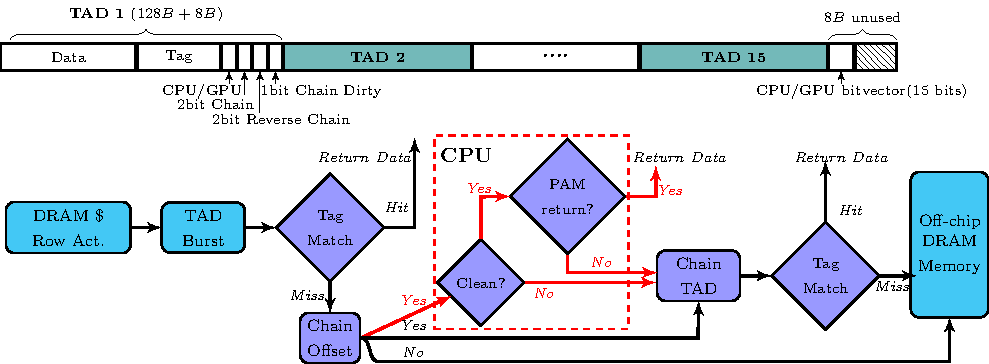
\includegraphics[scale=0.96]{figures/chaining}
	\caption{\cachename\ Row Organization and Access Path of a Request for \chaining}	
	\label{fig:chain-access}
\end{figure}

Additionally, each tag also stores 1 bit information about the owner of the block (CPU or GPU). This bit is used to make quick replacement decisions locally. The additional metadata required for \chaining\ is only 6 bits which can easily be accommodated in the existing 8 byte metadata. Lastly, the unused 8 byte (at the end of each row(page)) is used to store ownership information of each block in the row (15 bits). This information is used to make the \chaining\ replacement decision.


\par As explained earlier, when the \textit{$l_{cpu}$} threshold is reached, GPU lines are not allowed to evict CPU blocks and such GPU requests contending to evict a CPU line are forced to chain to another block belonging to a GPU and evicting that instead, thus maintaining the \textit{$l_{cpu}$} occupancy for CPU. In the very rare case that a GPU block is not found within the 3 consecutive locations the request is not inserted into the cache.

\begin{table}[htb]
	\centering
	\begin{tabular}{|c|c|c|c|c|}
\hline
\multirow{2}{*}{\begin{tabular}[c]{@{}l@{}}Threshold \\ Reached?\end{tabular}} & \multirow{2}{*}{\begin{tabular}[c]{@{}l@{}}Original\\ Set\end{tabular}} & \multirow{2}{*}{\begin{tabular}[c]{@{}l@{}}Not \\ Chained\end{tabular}} & \multicolumn{2}{c|}{Chained Set}                                                                                         \\ \cline{4-5} 
                                                                               &                                                                         &                                                                         & CPU                                                        & GPU                                                        \\ \hline
\multirow{2}{*}{No}                                                             & CPU                                                                     & \begin{tabular}[c]{@{}l@{}}replace\\ original\end{tabular}              & \begin{tabular}[c]{@{}l@{}}replace\\ chained\end{tabular}  & \begin{tabular}[c]{@{}l@{}}replace\\ original\end{tabular} \\ \cline{2-5} 
                                                                               & GPU                                                                     & \begin{tabular}[c]{@{}l@{}}Chain to\\ nearest \\ CPU set\end{tabular}   & \begin{tabular}[c]{@{}l@{}}replace\\ chained\end{tabular}  & \begin{tabular}[c]{@{}l@{}}replace\\ original\end{tabular} \\ \hline
\multirow{2}{*}{Yes}                                                             & CPU                                                                     & \begin{tabular}[c]{@{}l@{}}Chain to\\ nearest\\ GPU Set\end{tabular}    & \begin{tabular}[c]{@{}l@{}}do not\\ insert\end{tabular}    & \begin{tabular}[c]{@{}l@{}}replace\\ chained\end{tabular}  \\ \cline{2-5} 
                                                                               & GPU                                                                     & \begin{tabular}[c]{@{}l@{}}replace\\ original\end{tabular}              & \begin{tabular}[c]{@{}l@{}}replace\\ original\end{tabular} & \begin{tabular}[c]{@{}l@{}}replace\\ original\end{tabular} \\ \hline
\end{tabular}
	\caption{\chaining\ Mechanisms GPU Fill Request Insertion Policy}
	\label{chaining-replacement}
\end{table}

\subsubsection{Insertion Policy}
\par We now summarize the insertion policy used by \chaining\ mechanism in \cachename. 
\par For all CPU fill (insertion) requests, the data is always inserted in the original block, and the victim block is evicted. If the set that the CPU occupied  here is a \textit{chained block}, chaining is removed using the reverse chain bit i.e., the chain bits in the \textit{original block} are reset
\footnote{Additional bandwidth required for resetting chain bits in the \textit{original block} in this scenario has been accounted for in the simulation. We also account for the additional bandwidth required to occasionally access CPU/GPU bit vector at the end of the DRAM row. We find that the average bandwidth overhead for chaining across our benchmarks is just 4.7\%.}.
\par The memory controller maintains a running GPU occupancy counter for each row in the DRAM cache. This information is accommodated in the unused bits at the end of the row in the DRAM cache and can be cached in SRAM structures for fast lookups. Using this current occupancy counter the controller decides the fill policy for the GPU fill request. \cachename\ checks whether the threshold reached is determined by comparing the current GPU occupancy with the set \textit{$l_{cpu}$} threshold value as : $O_{gpu}\le(1-l_{cpu})$ where $O_{gpu}$ is the current GPU occupancy in the DRAM cache row. For a GPU fill request, if the low threshold mark for CPU occupancy is not reached, then the \chaining\ scheme replaces a CPU location, either from the original location or from the chained location, as indicated in row 1 of Table \ref{chaining-replacement}. For a GPU fill request, if the original location belongs to GPU and does not have a chained location, then block is inserted in one of the nearest CPU block [$(B+1)\%N_s$ or $(B+2)\%N_s$ or $(B+3)\%N_s$]. If such a nearest CPU block is not found, the request is inserted into original block itself. If the original location is chained, then the scheme replaces the chained location, if that belongs to CPU or the original location itself, as indicated in row 2 of Table \ref{chaining-replacement}. When the CPU occupancy has hit low threshold, then a GPU fill request replaces the original location if it belongs to GPU (row 4 in Table \ref{chaining-replacement}). If the original location belongs to CPU and does not have a chained block, then the GPU request is chained to the next nearest GPU location. If the original location is chained, but the chained location belongs to GPU, then the fill request replaces that. Otherwise, the fill request is not inserted in the DRAM cache (see row 3 in Table \ref{chaining-replacement}). Thus the \chaining\ scheme ensures, as far as possible, the CPU requests can find the data in the original location, while the GPU requests attempt to exploit pseudo-associativity for increased cache occupancy. In all cases (for both GPU and CPU requests) the access is satisfied with at most 2 tag matches, either in original location or in the chained location (identified by the chain bits). 

\par In essence, \cachename\ uses this \chaining\ mechanism to force occupancy control in the DRAM cache. \chaining\ is able to 
\begin{enumerate}[label=(\roman*)]
	\item ensure a minimum occupancy for the CPU lines while effectively allowing the GPU to occupy the rest of the DRAM cache by providing pseudo-associativity.
	\item remain as a direct mapped cache for majority of the CPU requests.
	\item avoid forcing eviction of hot GPU lines while also avoiding storing of dead lines in the cache.
\end{enumerate}

\subsubsection{\chaining\ Hardware Overhead}
This occupancy control mechanism does not incur any additional storage and uses the unused space in the DRAM cache rows. Once the GPU finishes kernel execution \cachename\ returns to a direct mapped cache as the CPU lines inserted into the DRAM cache occupy \textit{chained blocks} thereby unlinking chains. 

\section{Summary}
In this chapter, we presented the \cachename\ organization and mechanisms. We first showed the conscientious design decisions made and substantiated them with experiments of DRAM cache for IHS architecture. We then detail the principles and working of the three \cachename\ mechanisms - \prioname, \bypassname\ and \chaining. For each of the mechanisms, we describe the issues they try to address, describe their working in detail and the hardware overheads incurred. \cachename\ mechanisms are heterogeneity-aware, lightweight (incurring minimal or no hardware overhead) and can dynamically adapt to the inherent disparity of demands in an IHS architecture.

